% TU Eindhoven beamer template
% Author: Jens d'Hondt
% Eindhoven University of Technology

\documentclass{beamer}

\usepackage[english]{babel}
\usepackage{calc}
\usepackage[absolute,overlay]{textpos}
\usepackage{graphicx}

\usepackage{amsmath}
\usepackage{amsfonts}
\usepackage{mathtools}
\usepackage{comment}
\usepackage{MnSymbol,wasysym}
\usepackage{tikz}
\usepackage{subcaption}
%\usepackage{yhmath}
\usepackage{cancel}
\usepackage{color}
\usepackage{siunitx}
\usepackage{array}
\usepackage{multirow}
\usepackage{amssymb}
\usepackage{gensymb}
\usepackage{tabularx}
\usepackage{extarrows}
\usepackage{booktabs}
\usepackage{svg}
\usepackage[ruled,vlined]{algorithm2e}
%\setbeamertemplate{caption}[numbered]
\newcommand\mycommfont[1]{\footnotesize\ttfamily\textcolor{blue}{#1}}
\SetCommentSty{mycommfont}

\usepackage{physics}





\usetikzlibrary{fadings}
\usetikzlibrary{patterns}
\usetikzlibrary{shadows.blur}
\usetikzlibrary{shapes}



\input{content/math}




\setbeamertemplate{navigation symbols}{} % remove navigation symbols
\mode<presentation>{\usetheme{tue}}

% BIB SETTINGS
\usepackage[backend=bibtex,firstinits=true,maxnames=30,maxcitenames=20,url=false,style=authoryear]{biblatex}
\bibliography{bibfile}
\setlength\bibitemsep{0.3cm} % space between entries in the reference list
\renewcommand{\bibfont}{\normalfont\scriptsize}
\setbeamerfont{footnote}{size=\tiny}
\renewcommand{\cite}[1]{\footnote<.->[frame]{\fullcite{#1}}}


\title{S$\Omega$I: Score-based O-Information Estimation }
\institute{ \inst{1} EURECOM \inst{2} Ampere Software Technology , France}

\author{Mustapha Bounoua \inst{1}\inst{2} \and Giulio Franzese \inst{1} \and Pietro Michiardi \inst{1}}
%\date{}

\begin{document}



{
\setbeamertemplate{footline}{\usebeamertemplate*{minimal footline}}
\frame{\titlepage}
}

{\setbeamertemplate{footline}{\usebeamertemplate*{minimal footline}}

}

\begin{frame}{Introduction}

\begin{itemize}
    \item Complex systems are often described by \textbf{multivariate} information.
    \item Understanding the \textbf{relationships} among multiple random variables is crucial to analyse these systems.
    %\item Shannon Mutual information is not interpretable for $N>3$.
\end{itemize}

\begin{figure}
\begin{subfigure}{0.25\textwidth}
    %\centering
    

\tikzset{every picture/.style={line width=0.75pt}} %set default line width to 0.75pt        

\begin{tikzpicture}[x=0.75pt,y=0.75pt,yscale=-1,xscale=1,scale=0.6, every node/.style={scale=0.6}]
%uncomment if require: \path (0,293); %set diagram left start at 0, and has height of 293

%Image [id:dp5236848150513451] 

\draw (136.7,134.11) node  {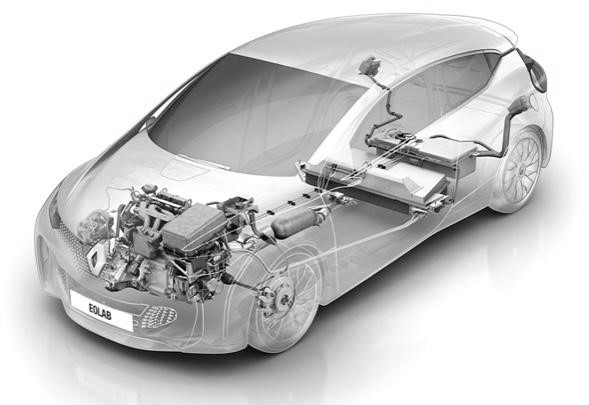
\includegraphics[width=204.75pt,height=138pt]{assets/cars.jpg}};
%Shape: Ellipse [id:dp22575039289402277] 
\draw  [color={rgb, 255:red, 255; green, 255; blue, 255 }  ,draw opacity=1 ][fill={rgb, 255:red, 255; green, 255; blue, 255 }  ,fill opacity=1 ] (11.33,122.73) .. controls (11.33,114.82) and (17.45,108.4) .. (25,108.4) .. controls (32.55,108.4) and (38.67,114.82) .. (38.67,122.73) .. controls (38.67,130.65) and (32.55,137.07) .. (25,137.07) .. controls (17.45,137.07) and (11.33,130.65) .. (11.33,122.73) -- cycle ;
%Shape: Ellipse [id:dp3623945699685074] 
\draw  [color={rgb, 255:red, 255; green, 255; blue, 255 }  ,draw opacity=1 ][fill={rgb, 255:red, 255; green, 255; blue, 255 }  ,fill opacity=1 ] (84.67,185.4) .. controls (84.67,177.48) and (90.79,171.07) .. (98.33,171.07) .. controls (105.88,171.07) and (112,177.48) .. (112,185.4) .. controls (112,193.32) and (105.88,199.73) .. (98.33,199.73) .. controls (90.79,199.73) and (84.67,193.32) .. (84.67,185.4) -- cycle ;
%Shape: Ellipse [id:dp8906821910938405] 
\draw  [color={rgb, 255:red, 255; green, 255; blue, 255 }  ,draw opacity=1 ][fill={rgb, 255:red, 255; green, 255; blue, 255 }  ,fill opacity=1 ] (207.33,53.4) .. controls (207.33,45.48) and (213.45,39.07) .. (221,39.07) .. controls (228.55,39.07) and (234.67,45.48) .. (234.67,53.4) .. controls (234.67,61.32) and (228.55,67.73) .. (221,67.73) .. controls (213.45,67.73) and (207.33,61.32) .. (207.33,53.4) -- cycle ;
%Shape: Ellipse [id:dp1843235766479494] 
\draw  [color={rgb, 255:red, 255; green, 255; blue, 255 }  ,draw opacity=1 ][fill={rgb, 255:red, 255; green, 255; blue, 255 }  ,fill opacity=1 ] (240.33,98.07) .. controls (240.33,90.15) and (246.45,83.73) .. (254,83.73) .. controls (261.55,83.73) and (267.67,90.15) .. (267.67,98.07) .. controls (267.67,105.98) and (261.55,112.4) .. (254,112.4) .. controls (246.45,112.4) and (240.33,105.98) .. (240.33,98.07) -- cycle ;
%Shape: Polygon Curved [id:ds2694891835945543] 
\draw  [draw opacity=0][fill={rgb, 255:red, 74; green, 145; blue, 158 }  ,fill opacity=0.25 ] (22.67,101.33) .. controls (32.67,96) and (57.33,94) .. (51.33,112) .. controls (45.33,130) and (50,119.33) .. (44,131.33) .. controls (38,143.33) and (27.33,164.67) .. (7.33,134.67) .. controls (-12.67,104.67) and (12.67,106.67) .. (22.67,101.33) -- cycle ;

%Shape: Polygon Curved [id:ds6576330285171925] 
\draw  [draw opacity=0][fill={rgb, 255:red, 139; green, 87; blue, 42 }  ,fill opacity=0.2 ] (96.67,166) .. controls (126.67,164.8) and (125.33,174.53) .. (119.33,192.53) .. controls (113.33,210.53) and (102,209.87) .. (94,210.53) .. controls (86,211.2) and (58.67,181.73) .. (67.33,177.87) .. controls (76,174) and (66.67,167.2) .. (96.67,166) -- cycle ;

%Shape: Polygon Curved [id:ds2775692663684084] 
\draw  [draw opacity=0][fill={rgb, 255:red, 206; green, 106; blue, 107 }  ,fill opacity=0.2 ] (248.33,75) .. controls (258.33,69.67) and (283,67.67) .. (277,85.67) .. controls (271,103.67) and (275.67,93) .. (269.67,105) .. controls (263.67,117) and (253,138.33) .. (233,108.33) .. controls (213,78.33) and (238.33,80.33) .. (248.33,75) -- cycle ;

%Shape: Polygon Curved [id:ds12005288403924697] 
\draw  [draw opacity=0][fill={rgb, 255:red, 245; green, 166; blue, 35 }  ,fill opacity=0.2 ] (138.4,48.87) .. controls (148.4,43.53) and (173.07,41.53) .. (167.07,59.53) .. controls (161.07,77.53) and (165.73,66.87) .. (159.73,78.87) .. controls (153.73,90.87) and (143.07,112.2) .. (123.07,82.2) .. controls (103.07,52.2) and (128.4,54.2) .. (138.4,48.87) -- cycle ;

%Shape: Polygon Curved [id:ds34961065781940404] 
\draw  [draw opacity=0][fill={rgb, 255:red, 190; green, 211; blue, 195 }  ,fill opacity=0.2 ] (217.07,33.2) .. controls (227.07,27.87) and (251.73,25.87) .. (245.73,43.87) .. controls (239.73,61.87) and (244.4,51.2) .. (238.4,63.2) .. controls (232.4,75.2) and (221.73,96.53) .. (201.73,66.53) .. controls (181.73,36.53) and (207.07,38.53) .. (217.07,33.2) -- cycle ;

%Shape: Ellipse [id:dp6562955430613056] 
\draw  [color={rgb, 255:red, 255; green, 255; blue, 255 }  ,draw opacity=1 ][fill={rgb, 255:red, 255; green, 255; blue, 255 }  ,fill opacity=1 ] (128.67,70.07) .. controls (128.67,62.15) and (134.79,55.73) .. (142.33,55.73) .. controls (149.88,55.73) and (156,62.15) .. (156,70.07) .. controls (156,77.98) and (149.88,84.4) .. (142.33,84.4) .. controls (134.79,84.4) and (128.67,77.98) .. (128.67,70.07) -- cycle ;

% Text Node
\draw  [draw opacity=0][fill={rgb, 255:red, 190; green, 211; blue, 195 }  ,fill opacity=0.2 ]  (222.07, 54.2) circle [x radius= 16.97, y radius= 15.56]   ;
\draw (211.07,45.6) node [anchor=north west][inner sep=0.75pt]    {$X^{2}$};
% Text Node
\draw  [draw opacity=0][fill={rgb, 255:red, 245; green, 166; blue, 35 }  ,fill opacity=0.2 ]  (143.4, 69.87) circle [x radius= 16.97, y radius= 15.56]   ;
\draw (132.4,61.27) node [anchor=north west][inner sep=0.75pt]    {$X^{3}$};
% Text Node
\draw  [draw opacity=0][fill={rgb, 255:red, 206; green, 106; blue, 107 }  ,fill opacity=0.2 ]  (253.33, 96) circle [x radius= 16.97, y radius= 15.56]   ;
\draw (242.33,87.4) node [anchor=north west][inner sep=0.75pt]    {$X^{4}$};
% Text Node
\draw  [draw opacity=0][fill={rgb, 255:red, 74; green, 145; blue, 158 }  ,fill opacity=0.35 ]  (27.67, 122.33) circle [x radius= 16.97, y radius= 15.56]   ;
\draw (16.67,113.73) node [anchor=north west][inner sep=0.75pt]    {$X^{1}$};
% Text Node
\draw  [draw opacity=0][fill={rgb, 255:red, 139; green, 87; blue, 42 }  ,fill opacity=0.2 ]  (100.33, 185) circle [x radius= 16.97, y radius= 15.56]   ;
\draw (89.33,176.4) node [anchor=north west][inner sep=0.75pt]    {$X^{5}$};


\end{tikzpicture}

    \caption*{Sensors}
\end{subfigure}
\begin{subfigure}{0.3\textwidth}
    %\centering
    %

\tikzset{every picture/.style={line width=0.75pt}} %set default line width to 0.75pt        

\begin{tikzpicture}[x=0.75pt,y=0.75pt,yscale=-1,xscale=1,scale=0.6, every node/.style={scale=0.6}]
%uncomment if require: \path (0,293); %set diagram left start at 0, and has height of 293

%Image [id:dp5236848150513451] 

\draw (136.7,134.11) node  {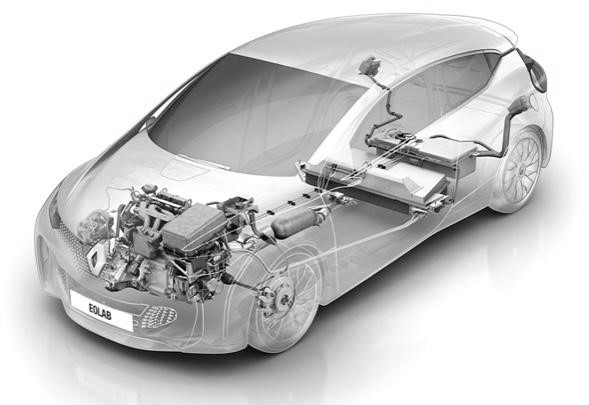
\includegraphics[width=204.75pt,height=138pt]{assets/cars.jpg}};
%Shape: Ellipse [id:dp22575039289402277] 
\draw  [color={rgb, 255:red, 255; green, 255; blue, 255 }  ,draw opacity=1 ][fill={rgb, 255:red, 255; green, 255; blue, 255 }  ,fill opacity=1 ] (11.33,122.73) .. controls (11.33,114.82) and (17.45,108.4) .. (25,108.4) .. controls (32.55,108.4) and (38.67,114.82) .. (38.67,122.73) .. controls (38.67,130.65) and (32.55,137.07) .. (25,137.07) .. controls (17.45,137.07) and (11.33,130.65) .. (11.33,122.73) -- cycle ;
%Shape: Ellipse [id:dp3623945699685074] 
\draw  [color={rgb, 255:red, 255; green, 255; blue, 255 }  ,draw opacity=1 ][fill={rgb, 255:red, 255; green, 255; blue, 255 }  ,fill opacity=1 ] (84.67,185.4) .. controls (84.67,177.48) and (90.79,171.07) .. (98.33,171.07) .. controls (105.88,171.07) and (112,177.48) .. (112,185.4) .. controls (112,193.32) and (105.88,199.73) .. (98.33,199.73) .. controls (90.79,199.73) and (84.67,193.32) .. (84.67,185.4) -- cycle ;
%Shape: Ellipse [id:dp8906821910938405] 
\draw  [color={rgb, 255:red, 255; green, 255; blue, 255 }  ,draw opacity=1 ][fill={rgb, 255:red, 255; green, 255; blue, 255 }  ,fill opacity=1 ] (207.33,53.4) .. controls (207.33,45.48) and (213.45,39.07) .. (221,39.07) .. controls (228.55,39.07) and (234.67,45.48) .. (234.67,53.4) .. controls (234.67,61.32) and (228.55,67.73) .. (221,67.73) .. controls (213.45,67.73) and (207.33,61.32) .. (207.33,53.4) -- cycle ;
%Shape: Ellipse [id:dp1843235766479494] 
\draw  [color={rgb, 255:red, 255; green, 255; blue, 255 }  ,draw opacity=1 ][fill={rgb, 255:red, 255; green, 255; blue, 255 }  ,fill opacity=1 ] (240.33,98.07) .. controls (240.33,90.15) and (246.45,83.73) .. (254,83.73) .. controls (261.55,83.73) and (267.67,90.15) .. (267.67,98.07) .. controls (267.67,105.98) and (261.55,112.4) .. (254,112.4) .. controls (246.45,112.4) and (240.33,105.98) .. (240.33,98.07) -- cycle ;
%Shape: Polygon Curved [id:ds2694891835945543] 
\draw  [draw opacity=0][fill={rgb, 255:red, 74; green, 145; blue, 158 }  ,fill opacity=0.25 ] (22.67,101.33) .. controls (32.67,96) and (57.33,94) .. (51.33,112) .. controls (45.33,130) and (50,119.33) .. (44,131.33) .. controls (38,143.33) and (27.33,164.67) .. (7.33,134.67) .. controls (-12.67,104.67) and (12.67,106.67) .. (22.67,101.33) -- cycle ;

%Shape: Polygon Curved [id:ds6576330285171925] 
\draw  [draw opacity=0][fill={rgb, 255:red, 139; green, 87; blue, 42 }  ,fill opacity=0.2 ] (96.67,166) .. controls (126.67,164.8) and (125.33,174.53) .. (119.33,192.53) .. controls (113.33,210.53) and (102,209.87) .. (94,210.53) .. controls (86,211.2) and (58.67,181.73) .. (67.33,177.87) .. controls (76,174) and (66.67,167.2) .. (96.67,166) -- cycle ;

%Shape: Polygon Curved [id:ds2775692663684084] 
\draw  [draw opacity=0][fill={rgb, 255:red, 206; green, 106; blue, 107 }  ,fill opacity=0.2 ] (248.33,75) .. controls (258.33,69.67) and (283,67.67) .. (277,85.67) .. controls (271,103.67) and (275.67,93) .. (269.67,105) .. controls (263.67,117) and (253,138.33) .. (233,108.33) .. controls (213,78.33) and (238.33,80.33) .. (248.33,75) -- cycle ;

%Shape: Polygon Curved [id:ds12005288403924697] 
\draw  [draw opacity=0][fill={rgb, 255:red, 245; green, 166; blue, 35 }  ,fill opacity=0.2 ] (138.4,48.87) .. controls (148.4,43.53) and (173.07,41.53) .. (167.07,59.53) .. controls (161.07,77.53) and (165.73,66.87) .. (159.73,78.87) .. controls (153.73,90.87) and (143.07,112.2) .. (123.07,82.2) .. controls (103.07,52.2) and (128.4,54.2) .. (138.4,48.87) -- cycle ;

%Shape: Polygon Curved [id:ds34961065781940404] 
\draw  [draw opacity=0][fill={rgb, 255:red, 190; green, 211; blue, 195 }  ,fill opacity=0.2 ] (217.07,33.2) .. controls (227.07,27.87) and (251.73,25.87) .. (245.73,43.87) .. controls (239.73,61.87) and (244.4,51.2) .. (238.4,63.2) .. controls (232.4,75.2) and (221.73,96.53) .. (201.73,66.53) .. controls (181.73,36.53) and (207.07,38.53) .. (217.07,33.2) -- cycle ;

%Shape: Ellipse [id:dp6562955430613056] 
\draw  [color={rgb, 255:red, 255; green, 255; blue, 255 }  ,draw opacity=1 ][fill={rgb, 255:red, 255; green, 255; blue, 255 }  ,fill opacity=1 ] (128.67,70.07) .. controls (128.67,62.15) and (134.79,55.73) .. (142.33,55.73) .. controls (149.88,55.73) and (156,62.15) .. (156,70.07) .. controls (156,77.98) and (149.88,84.4) .. (142.33,84.4) .. controls (134.79,84.4) and (128.67,77.98) .. (128.67,70.07) -- cycle ;

% Text Node
\draw  [draw opacity=0][fill={rgb, 255:red, 190; green, 211; blue, 195 }  ,fill opacity=0.2 ]  (222.07, 54.2) circle [x radius= 16.97, y radius= 15.56]   ;
\draw (211.07,45.6) node [anchor=north west][inner sep=0.75pt]    {$X^{2}$};
% Text Node
\draw  [draw opacity=0][fill={rgb, 255:red, 245; green, 166; blue, 35 }  ,fill opacity=0.2 ]  (143.4, 69.87) circle [x radius= 16.97, y radius= 15.56]   ;
\draw (132.4,61.27) node [anchor=north west][inner sep=0.75pt]    {$X^{3}$};
% Text Node
\draw  [draw opacity=0][fill={rgb, 255:red, 206; green, 106; blue, 107 }  ,fill opacity=0.2 ]  (253.33, 96) circle [x radius= 16.97, y radius= 15.56]   ;
\draw (242.33,87.4) node [anchor=north west][inner sep=0.75pt]    {$X^{4}$};
% Text Node
\draw  [draw opacity=0][fill={rgb, 255:red, 74; green, 145; blue, 158 }  ,fill opacity=0.35 ]  (27.67, 122.33) circle [x radius= 16.97, y radius= 15.56]   ;
\draw (16.67,113.73) node [anchor=north west][inner sep=0.75pt]    {$X^{1}$};
% Text Node
\draw  [draw opacity=0][fill={rgb, 255:red, 139; green, 87; blue, 42 }  ,fill opacity=0.2 ]  (100.33, 185) circle [x radius= 16.97, y radius= 15.56]   ;
\draw (89.33,176.4) node [anchor=north west][inner sep=0.75pt]    {$X^{5}$};


\end{tikzpicture}

    \hspace{1cm}
\end{subfigure}
\begin{subfigure}{0.25\textwidth}
    %\centering
    \input{assets/brain}
    \caption*{\newline Brain regions}
\end{subfigure}
\caption*{Is the sensors information redundant or complementary ? How different brain regions interact during a specific task ?}
\end{figure}
\end{frame}

%% Speech: In complex systems, multivariate information plays a crucial role in describing the interactions among its components. For instance, how do sensors in a robotic sytem share or complement information? Or, how do different brain regions interact during specific tasks? Answering these questions requires a deep understanding of multivariate relationships. We'll explore these dynamics and introduce our method for analyzing them




\begin{frame}{Extensions of Shannon Mutual information}

Shannon Mutual information is not interpretable for $N>3$. Some alternatives:
\newline
\begin{columns}
\begin{column}{.45\textwidth}
\textbf{PID}\cite{williams2010nonnegative}:
\begin{itemize}
    \item Requires a partition into sources and target.
    \item No common definition.
    \item Not scalable.
\end{itemize}
\end{column}
\begin{column}{.45\textwidth}
\textbf{O-information}\cite{Rosas2019QuantifyingHI}:
\begin{itemize}
    \item No partition needed.
    \item Derived from traditional\textit{ Information Theory} measures.
    \item Scalable.
\end{itemize}
\end{column}
\end{columns}
\end{frame}


%% Speech: Shannon Mutual Information is well-known, but its interpretability diminishes with more than three variables. Alternatives like Partial Information Decomposition (PID) and O-Information have been proposed. PID, while insightful, faces scalability issues and lacks a consensus definition. On the other hand, O-Information, derived from traditional Information Theory measures, offers a scalable solution without needing a partition into sources and targets.

\begin{frame}{Introduction}
\begin{columns}
\begin{column}{.45\textwidth}
\textit{\textbf{Redundancy }}: The \textbf{shared} information between subsets of the partition of variables.
\newline
\end{column}
\begin{column}{.45\textwidth}
\textit{\textbf{Synergy }}: The information observed by the \textbf{jointly} presence of variables but not available from individual alone.
\newline
\end{column}
\end{columns}
\begin{figure}
    \centering
    

\tikzset{every picture/.style={line width=0.75pt}} %set default line width to 0.75pt        

\begin{tikzpicture}[x=0.75pt,y=0.75pt,yscale=-1,xscale=1]
%uncomment if require: \path (0,300); %set diagram left start at 0, and has height of 300

%Shape: Ellipse [id:dp7373298723691162] 
\draw  [fill={rgb, 255:red, 206; green, 106; blue, 107 }  ,fill opacity=0.2 ][dash pattern={on 0.84pt off 2.51pt}] (71.4,159.3) .. controls (71.4,127.1) and (102.2,101) .. (140.2,101) .. controls (178.2,101) and (209,127.1) .. (209,159.3) .. controls (209,191.5) and (178.2,217.6) .. (140.2,217.6) .. controls (102.2,217.6) and (71.4,191.5) .. (71.4,159.3) -- cycle ;
%Shape: Circle [id:dp03598595550859773] 
\draw  [fill={rgb, 255:red, 74; green, 145; blue, 158 }  ,fill opacity=0.45 ] (71.4,156.3) .. controls (71.4,134.6) and (89,117) .. (110.7,117) .. controls (132.4,117) and (150,134.6) .. (150,156.3) .. controls (150,178) and (132.4,195.6) .. (110.7,195.6) .. controls (89,195.6) and (71.4,178) .. (71.4,156.3) -- cycle ;
%Shape: Circle [id:dp05882206005366952] 
\draw  [fill={rgb, 255:red, 190; green, 211; blue, 195 }  ,fill opacity=0.5 ] (130.4,156.3) .. controls (130.4,134.6) and (148,117) .. (169.7,117) .. controls (191.4,117) and (209,134.6) .. (209,156.3) .. controls (209,178) and (191.4,195.6) .. (169.7,195.6) .. controls (148,195.6) and (130.4,178) .. (130.4,156.3) -- cycle ;
%Shape: Circle [id:dp6392767984689582] 
\draw  [fill={rgb, 255:red, 34; green, 109; blue, 104 }  ,fill opacity=0.5 ] (104.4,178.3) .. controls (104.4,156.6) and (122,139) .. (143.7,139) .. controls (165.4,139) and (183,156.6) .. (183,178.3) .. controls (183,200) and (165.4,217.6) .. (143.7,217.6) .. controls (122,217.6) and (104.4,200) .. (104.4,178.3) -- cycle ;

% Text Node
\draw (83.45,148.97) node [anchor=north west][inner sep=0.75pt]  [font=\small,rotate=-359.65]  {$X^{1}$};
% Text Node
\draw (130.16,192.97) node [anchor=north west][inner sep=0.75pt]  [font=\small,rotate=-359.65]  {$X^{3}$};
% Text Node
\draw (185.9,149.47) node [anchor=north west][inner sep=0.75pt]  [font=\small,rotate=-359.65]  {$X^{2}$};
% Text Node
\draw  [draw opacity=0][fill={rgb, 255:red, 255; green, 255; blue, 255 }  ,fill opacity=0.5 ]  (122.7,103) -- (157.7,103) -- (157.7,117) -- (122.7,117) -- cycle  ;
\draw (125.7,107) node [anchor=north west][inner sep=0.75pt]  [font=\tiny,color={rgb, 255:red, 0; green, 0; blue, 0 }  ,opacity=1 ] [align=left] {Synergy};
% Text Node
\draw  [draw opacity=0][fill={rgb, 255:red, 255; green, 255; blue, 255 }  ,fill opacity=0.5 ]  (115.2,153.5) -- (165.2,153.5) -- (165.2,167.5) -- (115.2,167.5) -- cycle  ;
\draw (118.2,157.5) node [anchor=north west][inner sep=0.75pt]  [font=\tiny,color={rgb, 255:red, 0; green, 0; blue, 0 }  ,opacity=1 ] [align=left] {Redundancy};


\end{tikzpicture}

\end{figure}
\end{frame}



%% Speech : To understand complex interactions, it's essential to distinguish between redundancy and synergy. Redundancy refers to the shared information between variable subsets, while synergy captures the information that emerges only when variables are considered together. For example, consider how different sensors or brain regions might display these properties during specific tasks


\begin{frame}{High dimensional interaction measures}

$X = \{ \underbrace{ X^1,\dots,X^{i-1}}_{X^{<i} } ,X^i,\underbrace{X^{i+1},\dots,X^N}_{X^{>i}}  \} $ and $X^{\setminus i}=\{X^{<i},X^{>i}\}$.



\begin{itemize}

\item S-information: $   \cS(X) \defeq \sum\limits_{i=1}^N \cI(X^i;X^{\setminus i})$.

The total mutual information between one variable and the rest of the system. It accepts the following decomposition : $\cS(X)=\sum\limits_{i=1}^N \cI(X^i;X^{>i})+\sum\limits_{i=1}^N \cI(X^i;X^{<i} \g X^{>i})$.

\end{itemize}
\end{frame}

% speech :  Introducing S-Information, which sums up the mutual information between each variable and the rest of the system. This measure helps us understand how much information a single variable holds about the entire system. The decomposition of S-Information into total correlation and dual total correlation further refines this understanding.


\begin{frame}{High dimensional interaction measures}
\begin{itemize}

\item Total correlation: $\cT(X) = \sum\limits_{i=1}^N \cI(X^i;X^{>i})$. 
    
    How much information each variable $X^i$, \textbf{shares} with $ X^{>i}$ which suggests \textit{redundancy} markers.
\item Dual total correlation: $\cD( X) = \sum\limits_{i=1}^N \cI(X^i;X^{<i} \g X^{>i})$.

How much \textbf{additional} information the variables $X^{<i}$ carry about $X^i$ if  $ X^{>i}$ is also available suggests a \textit{synergistic} scenario.
\end{itemize}
\end{frame}

%% speech : Total correlation and dual total correlation offer two perspectives. Total correlation measures how much each variable shares information with the rest, indicating redundancy. Dual total correlation, however, shows the additional information a subset of variables holds about a particular variable, suggesting synergy. These measures help identify redundancy and synergy markers in complex systems."



\begin{frame}{O-information}




\begin{equation*}
  \Omega(X)=\cT(X)-\cD(X)
\end{equation*}

\begin{columns}
\begin{column}{.45\textwidth}
\begin{itemize}
    \item $\Omega(X)> 0 $ Redundancy dominance.
    \item $\Omega(X)< 0 $ Synergy dominance.
\end{itemize}
\end{column}
\begin{column}{.45\textwidth}

\begin{figure}
    \centering
    

\tikzset{every picture/.style={line width=0.75pt}} %set default line width to 0.75pt        

\begin{tikzpicture}[x=0.75pt,y=0.75pt,yscale=-1,xscale=1]
%uncomment if require: \path (0,293); %set diagram left start at 0, and has height of 293

%Image [id:dp7777581298700516] 
\draw (151.33,97) node   {\includesvg[width=163pt,height=119.5pt]{assets/brainsvg.svg}};
%Shape: Polygon Curved [id:ds34961065781940404] 
\draw  [draw opacity=0][fill={rgb, 255:red, 128; green, 128; blue, 128 }  ,fill opacity=0.2 ] (157.33,22.83) .. controls (167.33,17.5) and (192,15.5) .. (186,33.5) .. controls (180,51.5) and (184.67,40.83) .. (178.67,52.83) .. controls (172.67,64.83) and (162,86.17) .. (142,56.17) .. controls (122,26.17) and (147.33,28.17) .. (157.33,22.83) -- cycle ;

%Shape: Polygon Curved [id:ds12005288403924697] 
\draw  [draw opacity=0][fill={rgb, 255:red, 155; green, 155; blue, 155 }  ,fill opacity=0.2 ] (122.67,125.33) .. controls (132.67,120) and (157.33,118) .. (151.33,136) .. controls (145.33,154) and (150,143.33) .. (144,155.33) .. controls (138,167.33) and (127.33,188.67) .. (107.33,158.67) .. controls (87.33,128.67) and (112.67,130.67) .. (122.67,125.33) -- cycle ;

%Shape: Polygon Curved [id:ds2775692663684084] 
\draw  [draw opacity=0][fill={rgb, 255:red, 155; green, 155; blue, 155 }  ,fill opacity=0.2 ] (210,50) .. controls (220,44.67) and (244.67,42.67) .. (238.67,60.67) .. controls (232.67,78.67) and (237.33,68) .. (231.33,80) .. controls (225.33,92) and (214.67,113.33) .. (194.67,83.33) .. controls (174.67,53.33) and (200,55.33) .. (210,50) -- cycle ;

%Shape: Polygon Curved [id:ds2694891835945543] 
\draw  [draw opacity=0][fill={rgb, 255:red, 155; green, 155; blue, 155 }  ,fill opacity=0.2 ] (80.67,48) .. controls (90.67,42.67) and (115.33,40.67) .. (109.33,58.67) .. controls (103.33,76.67) and (108,66) .. (102,78) .. controls (96,90) and (85.33,111.33) .. (65.33,81.33) .. controls (45.33,51.33) and (70.67,53.33) .. (80.67,48) -- cycle ;

%Shape: Ellipse [id:dp22575039289402277] 
\draw  [color={rgb, 255:red, 255; green, 255; blue, 255 }  ,draw opacity=1 ][fill={rgb, 255:red, 255; green, 255; blue, 255 }  ,fill opacity=1 ] (73.33,69.4) .. controls (73.33,61.48) and (79.45,55.07) .. (87,55.07) .. controls (94.55,55.07) and (100.67,61.48) .. (100.67,69.4) .. controls (100.67,77.32) and (94.55,83.73) .. (87,83.73) .. controls (79.45,83.73) and (73.33,77.32) .. (73.33,69.4) -- cycle ;
%Shape: Ellipse [id:dp3623945699685074] 
\draw  [color={rgb, 255:red, 255; green, 255; blue, 255 }  ,draw opacity=1 ][fill={rgb, 255:red, 255; green, 255; blue, 255 }  ,fill opacity=1 ] (116,145.4) .. controls (116,137.48) and (122.12,131.07) .. (129.67,131.07) .. controls (137.21,131.07) and (143.33,137.48) .. (143.33,145.4) .. controls (143.33,153.32) and (137.21,159.73) .. (129.67,159.73) .. controls (122.12,159.73) and (116,153.32) .. (116,145.4) -- cycle ;
%Shape: Ellipse [id:dp4899964637813463] 
\draw  [color={rgb, 255:red, 255; green, 255; blue, 255 }  ,draw opacity=1 ][fill={rgb, 255:red, 255; green, 255; blue, 255 }  ,fill opacity=1 ] (146.67,44.73) .. controls (146.67,36.82) and (152.79,30.4) .. (160.33,30.4) .. controls (167.88,30.4) and (174,36.82) .. (174,44.73) .. controls (174,52.65) and (167.88,59.07) .. (160.33,59.07) .. controls (152.79,59.07) and (146.67,52.65) .. (146.67,44.73) -- cycle ;
%Shape: Ellipse [id:dp8906821910938405] 
\draw  [color={rgb, 255:red, 255; green, 255; blue, 255 }  ,draw opacity=1 ][fill={rgb, 255:red, 255; green, 255; blue, 255 }  ,fill opacity=1 ] (202.67,72.07) .. controls (202.67,64.15) and (208.79,57.73) .. (216.33,57.73) .. controls (223.88,57.73) and (230,64.15) .. (230,72.07) .. controls (230,79.98) and (223.88,86.4) .. (216.33,86.4) .. controls (208.79,86.4) and (202.67,79.98) .. (202.67,72.07) -- cycle ;
%Shape: Ellipse [id:dp1843235766479494] 
\draw  [color={rgb, 255:red, 255; green, 255; blue, 255 }  ,draw opacity=1 ][fill={rgb, 255:red, 255; green, 255; blue, 255 }  ,fill opacity=1 ] (200,122.73) .. controls (200,114.82) and (206.12,108.4) .. (213.67,108.4) .. controls (221.21,108.4) and (227.33,114.82) .. (227.33,122.73) .. controls (227.33,130.65) and (221.21,137.07) .. (213.67,137.07) .. controls (206.12,137.07) and (200,130.65) .. (200,122.73) -- cycle ;
%Shape: Polygon Curved [id:ds6576330285171925] 
\draw  [draw opacity=0][fill={rgb, 255:red, 155; green, 155; blue, 155 }  ,fill opacity=0.2 ] (212,102.67) .. controls (242,101.47) and (240.67,111.2) .. (234.67,129.2) .. controls (228.67,147.2) and (217.33,146.53) .. (209.33,147.2) .. controls (201.33,147.87) and (174,118.4) .. (182.67,114.53) .. controls (191.33,110.67) and (182,103.87) .. (212,102.67) -- cycle ;


% Text Node
\draw  [draw opacity=0][fill={rgb, 255:red, 128; green, 128; blue, 128 }  ,fill opacity=0.2 ]  (162.33, 43.83) circle [x radius= 16.97, y radius= 15.56]   ;
\draw (151.33,35.23) node [anchor=north west][inner sep=0.75pt]    {$X^{2}$};
% Text Node
\draw  [draw opacity=0][fill={rgb, 255:red, 155; green, 155; blue, 155 }  ,fill opacity=0.2 ]  (127.67, 146.33) circle [x radius= 16.97, y radius= 15.56]   ;
\draw (116.67,137.73) node [anchor=north west][inner sep=0.75pt]    {$X^{3}$};
% Text Node
\draw  [draw opacity=0][fill={rgb, 255:red, 155; green, 155; blue, 155 }  ,fill opacity=0.2 ]  (215, 71) circle [x radius= 16.97, y radius= 15.56]   ;
\draw (204,62.4) node [anchor=north west][inner sep=0.75pt]    {$X^{5}$};
% Text Node
\draw  [draw opacity=0][fill={rgb, 255:red, 155; green, 155; blue, 155 }  ,fill opacity=0.2 ]  (85.67, 69) circle [x radius= 16.97, y radius= 15.56]   ;
\draw (74.67,60.4) node [anchor=north west][inner sep=0.75pt]    {$X^{1}$};
% Text Node
\draw  [draw opacity=0][fill={rgb, 255:red, 155; green, 155; blue, 155 }  ,fill opacity=0.2 ]  (215.67, 121.67) circle [x radius= 16.97, y radius= 15.56]   ;
\draw (204.67,113.07) node [anchor=north west][inner sep=0.75pt]    {$X^{4}$};


\end{tikzpicture}

\end{figure}

\end{column}
\end{columns}
\end{frame}

%% O-Information is calculated as the difference between total correlation and dual total correlation. A positive O-Information indicates redundancy dominance, while a negative value suggests synergy dominance. This measure gives us a clearer picture of the interaction dynamics within a system."


\begin{frame}{Gradient of O-information}
\begin{columns}
\begin{column}{.45\textwidth}
The individual influence of each variable to the overall structure can be captured via the gradient of O-information:

\begin{equation*}
    \partial_i \Omega( X) =  \Omega( X) - \Omega( X^{\setminus i})
\end{equation*}
\end{column}
\begin{column}{.45\textwidth}
\begin{figure}
    \centering
    \tikzset{every picture/.style={line width=0.75pt}} %set default line width to 0.75pt        

\begin{tikzpicture}[x=0.75pt,y=0.75pt,yscale=-1,xscale=1]
%uncomment if require: \path (0,293); %set diagram left start at 0, and has height of 293

%Image [id:dp7777581298700516] 
\draw (151.33,97) node  {\includesvg[width=163pt,height=119.5pt]{assets/brainsvg.svg}};
%Shape: Polygon Curved [id:ds18393926555266948] 
\draw  [draw opacity=0][fill={rgb, 255:red, 206; green, 106; blue, 107 }  ,fill opacity=0.4 ] (66,71.67) .. controls (86.13,47.55) and (84.8,88.22) .. (109.47,109.55) .. controls (134.13,130.88) and (150.13,94.22) .. (170.13,124.22) .. controls (190.13,154.22) and (99.47,166.88) .. (76.13,131.55) .. controls (52.8,96.22) and (45.87,95.78) .. (66,71.67) -- cycle ;
%Shape: Polygon Curved [id:ds5930593507912458] 
\draw  [draw opacity=0][fill={rgb, 255:red, 74; green, 145; blue, 158 }  ,fill opacity=0.4 ] (109.47,50.08) .. controls (114.13,33.42) and (192.8,33.42) .. (208.13,45.55) .. controls (223.47,57.68) and (246.8,106.88) .. (241.47,127.55) .. controls (236.13,148.22) and (199.47,99.42) .. (188.8,118.75) .. controls (184.88,125.85) and (172.5,120.72) .. (158.64,110.55) .. controls (134.77,93.04) and (106.51,60.63) .. (109.47,50.08) -- cycle ;
%Shape: Circle [id:dp1678818803252513] 
\draw  [draw opacity=0][fill={rgb, 255:red, 255; green, 255; blue, 255 }  ,fill opacity=1 ] (64.21,98.63) .. controls (64.05,91.62) and (69.6,85.8) .. (76.62,85.64) .. controls (83.63,85.47) and (89.45,91.03) .. (89.61,98.04) .. controls (89.77,105.06) and (84.22,110.88) .. (77.2,111.04) .. controls (70.19,111.2) and (64.37,105.65) .. (64.21,98.63) -- cycle ;
%Shape: Circle [id:dp6869227528745232] 
\draw  [draw opacity=0][fill={rgb, 255:red, 255; green, 255; blue, 255 }  ,fill opacity=1 ] (138.21,133.97) .. controls (138.05,126.95) and (143.6,121.13) .. (150.62,120.97) .. controls (157.63,120.81) and (163.45,126.36) .. (163.61,133.38) .. controls (163.77,140.39) and (158.22,146.21) .. (151.2,146.37) .. controls (144.19,146.54) and (138.37,140.98) .. (138.21,133.97) -- cycle ;
%Shape: Circle [id:dp5438595708004899] 
\draw  [draw opacity=0][fill={rgb, 255:red, 255; green, 255; blue, 255 }  ,fill opacity=1 ] (93.54,135.3) .. controls (93.38,128.29) and (98.93,122.47) .. (105.95,122.3) .. controls (112.96,122.14) and (118.78,127.7) .. (118.95,134.71) .. controls (119.11,141.73) and (113.55,147.55) .. (106.54,147.71) .. controls (99.52,147.87) and (93.7,142.32) .. (93.54,135.3) -- cycle ;
%Shape: Circle [id:dp6212121433012971] 
\draw  [draw opacity=0][fill={rgb, 255:red, 255; green, 255; blue, 255 }  ,fill opacity=1 ] (121.54,57.97) .. controls (121.38,50.95) and (126.93,45.13) .. (133.95,44.97) .. controls (140.96,44.81) and (146.78,50.36) .. (146.95,57.38) .. controls (147.11,64.39) and (141.55,70.21) .. (134.54,70.37) .. controls (127.52,70.54) and (121.7,64.98) .. (121.54,57.97) -- cycle ;
%Shape: Circle [id:dp7627341450544065] 
\draw  [draw opacity=0][fill={rgb, 255:red, 255; green, 255; blue, 255 }  ,fill opacity=1 ] (206.87,101.3) .. controls (206.71,94.29) and (212.27,88.47) .. (219.28,88.3) .. controls (226.3,88.14) and (232.12,93.7) .. (232.28,100.71) .. controls (232.44,107.73) and (226.89,113.55) .. (219.87,113.71) .. controls (212.86,113.87) and (207.04,108.32) .. (206.87,101.3) -- cycle ;
%Shape: Circle [id:dp1869737705120207] 
\draw  [draw opacity=0][fill={rgb, 255:red, 255; green, 255; blue, 255 }  ,fill opacity=1 ] (172.87,69.3) .. controls (172.71,62.29) and (178.27,56.47) .. (185.28,56.3) .. controls (192.3,56.14) and (198.12,61.7) .. (198.28,68.71) .. controls (198.44,75.73) and (192.89,81.55) .. (185.87,81.71) .. controls (178.86,81.87) and (173.04,76.32) .. (172.87,69.3) -- cycle ;

% Text Node
\draw  [draw opacity=0][fill={rgb, 255:red, 206; green, 106; blue, 107 }  ,fill opacity=0.41 ]  (151, 133) circle [x radius= 16.97, y radius= 15.56]   ;
\draw (140,124.4) node [anchor=north west][inner sep=0.75pt]    {$X^{4}$};
% Text Node
\draw  [draw opacity=0][fill={rgb, 255:red, 206; green, 106; blue, 107 }  ,fill opacity=0.41 ]  (75.67, 98.33) circle [x radius= 16.97, y radius= 15.56]   ;
\draw (64.67,89.73) node [anchor=north west][inner sep=0.75pt]    {$X^{1}$};
% Text Node
\draw  [draw opacity=0][fill={rgb, 255:red, 206; green, 106; blue, 107 }  ,fill opacity=0.41 ]  (106.33, 135) circle [x radius= 16.97, y radius= 15.56]   ;
\draw (95.33,126.4) node [anchor=north west][inner sep=0.75pt]    {$X^{5}$};
% Text Node
\draw  [draw opacity=0][fill={rgb, 255:red, 74; green, 145; blue, 158 }  ,fill opacity=0.4 ]  (134.33, 57.67) circle [x radius= 16.97, y radius= 15.56]   ;
\draw (123.33,49.07) node [anchor=north west][inner sep=0.75pt]    {$X^{3}$};
% Text Node
\draw  [draw opacity=0][fill={rgb, 255:red, 74; green, 145; blue, 158 }  ,fill opacity=0.4 ]  (187, 68.33) circle [x radius= 16.97, y radius= 15.56]   ;
\draw (176,59.73) node [anchor=north west][inner sep=0.75pt]    {$X^{2}$};
% Text Node
\draw  [draw opacity=0][fill={rgb, 255:red, 74; green, 145; blue, 158 }  ,fill opacity=0.4 ]  (219, 99.67) circle [x radius= 16.97, y radius= 15.56]   ;
\draw (208,91.07) node [anchor=north west][inner sep=0.75pt]    {$X^{6}$};
% Text Node
\draw  [draw opacity=0][fill={rgb, 255:red, 206; green, 106; blue, 107 }  ,fill opacity=0.41 ]  (50.33,178) -- (126.33,178) -- (126.33,200) -- (50.33,200) -- cycle  ;
\draw (53.33,182.4) node [anchor=north west][inner sep=0.75pt]  [font=\footnotesize]  {$\partial _{i} \ \Omega ( X) < 0$};
% Text Node
\draw  [draw opacity=0][fill={rgb, 255:red, 74; green, 145; blue, 158 }  ,fill opacity=0.5 ]  (156.33,178) -- (232.33,178) -- (232.33,200) -- (156.33,200) -- cycle  ;
\draw (159.33,182.4) node [anchor=north west][inner sep=0.75pt]  [font=\footnotesize]  {$\partial _{i} \ \Omega ( X)  >0$};


\end{tikzpicture}

\end{figure}

\end{column}
\end{columns}
\end{frame}


%% speech The gradient of O-Information reveals the influence of individual variables on the overall structure. By examining the change in O-Information when a specific variable is removed, we can understand its contribution to redundancy or synergy within the system

\begin{frame}{Score-based KL Divergence estimation}

Let $X$ a random variable and $X_t= X + \sqrt{2t} W$ its noised version with an intensity indexed by $t\in[0,\infty)$. Using results from \cite{minde}:

\begin{align*}
    \KL{p(x)}{q(x)} &= \int p(x)\log\left(\frac{p(x)}{q(x)}\right) \dd x. \\
   &= \int p_{t}(x)\norm{\nabla \log p_{t}(x) - \nabla \log q_{t}(x) }^2\dd x\dd t
\end{align*}

\begin{itemize}
    \item All what we need is the time-varying score functions $\nabla \log(p_t)$ and $\nabla \log(q_t)$.
    \item Learning the score function by learning to denoise $X_t$ : $\nabla \log{p_{t}(x)}=\frac{\E[X\g X_t=x]-x}{2t} $. \textit{Any score based model\cite{song2021a} can be used. }
    
\end{itemize}
\end{frame}

%% By considering a noising process X_t illustrated here. A nice result form fransese 2024, the KL Divergence can be computed using difference of time-varying score function. To learn the score function, one can adopt the parameterization of learning a denoiser that denoise X_t back to X.

\begin{frame}{Score-based O-information estimation}
Let a multivariate random variable $X=\{X^{1},\dots,X^{N}\} \sim p(x^1,\dots,x^N)$:

\begin{align*} 
\cT(X)&=  \KL{p(x)}{\prod\limits_{i=1}^N p(x^i)} \\
&= \int \frac{1}{4t^2}\E\norm{\E[X\g X_t]-
      \begin{bmatrix}
          \E[X^i\g X^i_t]
      \end{bmatrix}_{i=1}^{N}}^2\dd t.   
\end{align*}

\begin{itemize}
\item Comparing the denoiser output when all the variables are denoised \textbf{together} (\textit{Joint}) or \textbf{separately} (\textit{Marginals}).
\end{itemize}
\end{frame}

%% Lets now use this results to estimate our measure of interest : TC can be written in terms of KL, by plug in the denoiser instead of the score we can obtain the following formulation which make a lot of sense. As TC is the difference between he denoiser outputs when variables are denoised together versus separately. So if the variables are not correlated the output is the same so KL is null.


\begin{frame}{Score-based O-information estimation}
%Dual total correlation can be also computed with the help of the denoising score functions . 
\begin{equation*}
\cD(X)  = \int \frac{1}{4t^2}\E\norm{\E[X\g X_t]-
        \begin{bmatrix}
            \E[X^i\g X^i_t, X^{\setminus i}]
        \end{bmatrix}_{i=1}^{N}}^2\dd t 
 \end{equation*}

\begin{itemize}
    \item Comparing the denoiser output when all the variables are denoised \textbf{together} (\textit{Joint}) or the individual denoising \textbf{conditioned} on the remaining clean variable (\textit{Conditionals}).
\end{itemize}

%% Similarly we can obtain a DTC formulation : we compare the denoiser output together (Joint) or the individual denoising conditioned on clean variables.

\begin{equation*}
  \Omega(X)=\cT(X)-\cD(X)
\end{equation*}
%% Now that we have TC and DTC, please recall that o-inf = T-D.


\begin{itemize}
    \item Gradient of O-information can be computed equivalently by computing $\Omega(X^{\setminus i})$.
\end{itemize}
\end{frame}

%% Gradient of O-information computation can be done equivalently by learning to compute.


\begin{frame}{Amortized approach using a unique network}


\begin{figure}
    \centering
    

\tikzset{every picture/.style={line width=0.75pt}} %set default line width to 0.75pt        

\begin{tikzpicture}[x=0.75pt,y=0.75pt,yscale=-1,xscale=1]
%uncomment if require: \path (0,300); %set diagram left start at 0, and has height of 300

%Rounded Rect [id:dp24071416230204656] 
\draw  [color={rgb, 255:red, 74; green, 74; blue, 74 }  ,draw opacity=1 ][fill={rgb, 255:red, 155; green, 155; blue, 155 }  ,fill opacity=0.3 ] (168.2,80.57) .. controls (168.2,74.42) and (173.18,69.43) .. (179.33,69.43) -- (271.57,69.43) .. controls (277.72,69.43) and (282.7,74.42) .. (282.7,80.57) -- (282.7,113.97) .. controls (282.7,120.12) and (277.72,125.1) .. (271.57,125.1) -- (179.33,125.1) .. controls (173.18,125.1) and (168.2,120.12) .. (168.2,113.97) -- cycle ;
%Straight Lines [id:da22602744857176815] 
\draw    (123.87,94.45) -- (165.87,94.93) ;
\draw [shift={(167.87,94.95)}, rotate = 180.65] [color={rgb, 255:red, 0; green, 0; blue, 0 }  ][line width=0.75]    (10.93,-3.29) .. controls (6.95,-1.4) and (3.31,-0.3) .. (0,0) .. controls (3.31,0.3) and (6.95,1.4) .. (10.93,3.29)   ;
%Straight Lines [id:da9408345556253781] 
\draw    (283.2,94.45) -- (319.7,94.92) ;
\draw [shift={(321.7,94.95)}, rotate = 180.74] [color={rgb, 255:red, 0; green, 0; blue, 0 }  ][line width=0.75]    (10.93,-3.29) .. controls (6.95,-1.4) and (3.31,-0.3) .. (0,0) .. controls (3.31,0.3) and (6.95,1.4) .. (10.93,3.29)   ;
%Straight Lines [id:da18925853941384863] 
\draw    (118.32,131.62) -- (185.7,132.36) ;
%Straight Lines [id:da39360099253546355] 
\draw    (185.7,124.93) -- (185.6,132.81) ;

% Text Node
\draw (102.03,73.02) node [anchor=north west][inner sep=0.75pt]  [font=\scriptsize]  {$ \begin{array}{l}
X_{t}^{1}\\
\ \vdots \\
X_{t}^{N}
\end{array}$};
% Text Node
\draw (325.2,67.35) node [anchor=north west][inner sep=0.75pt]  [font=\scriptsize]  {$ \begin{array}{l}
\epsilon _{\theta }\left( X_{t}^{1}\right)\\
\ \vdots \\
\epsilon _{\theta }\left( X_{t}^{N}\right)
\end{array}$};
% Text Node
\draw (221.94,94.45) node  [font=\footnotesize]  {$ \begin{array}{l}
\textcolor[rgb]{0.29,0.29,0.29}{Denoising}\\
\textcolor[rgb]{0.29,0.29,0.29}{\ \ \ \ Score\ }
\end{array}$};
% Text Node
\draw (104.57,120.8) node [anchor=north west][inner sep=0.75pt]    {$t$};


\end{tikzpicture}

\end{figure}

\begin{algorithm}[H]
\small
\caption{S$\Omega$I test-time}
\DontPrintSemicolon
\textbf{Input:} $ X = \{X^i\}_{i=1}^N, t \sim \mathcal{U}[0,T], \quad X_t \sim p_t $  \\
$ s_t(X_t) \gets \epsilon_\theta([X_t^1,\dots, X_t^N ], \tau = [t,\dots,t] ) $ \tcp{The joint}
\For{i = 1 \textbf{to} $N$ }{

$ s_t(X^i_t | X^{\setminus i} ) \gets \epsilon_\theta \left([X^1,..,X^i_t,..,X^N ],\tau = [0,..,t,..,0]\right) $ \tcp{ Conditional}
$ s_t(X^i_t) \gets \epsilon_\theta([X_T^1,\dots,X_t^i,\dots, X_T^N ], \tau = [T,..,t,..,T] ) $ \tcp{Marginal}%\footnote[]{The non marginal variables can be replaced with a Null vector adhering to a transformer based approach.}}
}
% $ \hat{\cT}(X) \gets \frac{g^2_t}{2} \norm{ s_t(X_t) - \left[ s_t(X^i_t) \right]_{i=1}^{N} }^2  $  \\
% $ \hat{\cD}(X) \gets \frac{g^2_t}{2} \norm{ s_t(X_t) - \left[ s_t(X^i_t | X^{\setminus i} ) \right]_{i=1}^{N} }^2  $  \\
% \textbf{Return} $ \hat{\Omega}(X) \gets \hat{\cT}(X)  - \hat{\cD}(X) $

\textbf{Return} $ \underbrace{ \frac{g^2_t}{2} \norm{ s_t(X_t) - \left[ s_t(X^i_t) \right]_{i=1}^{N} }^2 }_{\cT(X)}- \underbrace{\frac{g^2_t}{2} \norm{ s_t(X_t) - \left[ s_t(X^i_t | X^{\setminus i} ) \right]_{i=1}^{N} }^2 }_{\cD(X)}$

\end{algorithm}

%% We use a single score network for both joint and conditional and marginal denoising. We can use a multitime vector as well as maskin mechanisme to parmaetrize the model to render all the modes.



\end{frame}



% \begin{frame}{Synthetic benchmarks - $\Omega(X)$}

% \begin{columns}

% \begin{column}{.40\textwidth}
%     \begin{itemize}
%     \item \textbf{Redundancy}
%     $R \sim \mathcal{N}(0,\mathbb{I})$ is the \textit{redundant} information. $X = \{R + \epsilon_i,\dots, R + \epsilon_N\}$, where $\epsilon_i \sim \mathcal{N}(0,\sigma \mathbb{I})$ 
    
%  \item \textbf{Synergy:} let $ S \sim \mathcal{N}(0,\mathbb{I})$ be the \textit{synergistic} information. $ X^1 \sim \mathcal{N}(0, \mathbb{I})$,  $ X^2 = X^1 +  S $  ,$  X^3 =  S + \epsilon ,$ with $  \epsilon \sim \mathcal{N}(0,\sigma) $ and $ X^1 \indep X^3 
%     $
%        \end{itemize}
%     \end{column}
%     \begin{column}{.5\textwidth}
%     \begin{figure}
%     \centering
%         \begin{subfigure}[]{0.6\textwidth}
%                 \includegraphics[width=\textwidth]{assets/figures/exp_red/legend.PNG}
%             \end{subfigure}
            
%             \begin{subfigure}[]{0.6\textwidth}
%                 \includegraphics[width=\textwidth]{assets/figures/exp_red/plot_red_0_dim_20.jpg}
%             \end{subfigure}
            
%             \begin{subfigure}[]{0.6\textwidth}
%                 \includegraphics[width=\textwidth]{assets/figures/exp_red/plot_syn_0_dim_20.jpg}
%             \end{subfigure}
% \caption*{System of \textbf{10} variables of $Dim=20$ each: \textbf{Top}: Redundancy, \textbf{Bottom:} Synergy.}
% \end{figure}

%     \end{column}
% \end{columns}
% %% We tested our method on synthetic data. For redundancy, we generated variables with shared noise components. For synergy, we created variables that interact only when considered together. We considered here as baseline the bruteforce approach where each MI term in TC and DTC is estimated using a neural estimator. Our results, visualized here, show the outperformance of SOI.




% \end{frame}

% \begin{frame}{Synthetic benchmarks- $\partial \Omega(X)$}

%  \begin{figure}
%     \centering
%         \begin{subfigure}[]{0.45\textwidth}
%                 \includegraphics[width=\textwidth]{assets/figures/grad/grad_tx_setting_0_dim_20.png}
%             \end{subfigure}
%             \begin{subfigure}[]{0.45\textwidth}
%                 \includegraphics[width=\textwidth]{assets/figures/grad/grad_tx_setting_1_dim_20.png}
%             \end{subfigure}
            
%             \begin{subfigure}[]{0.45\textwidth}
%                \centering
%                \input{assets/6var_mix}
%             \end{subfigure}
%                 \begin{subfigure}[]{0.45\textwidth}
%                \centering
%                

\tikzset{every picture/.style={line width=0.75pt}} %set default line width to 0.75pt        

\begin{tikzpicture}[x=0.75pt,y=0.75pt,yscale=-1,xscale=1]
%uncomment if require: \path (0,293); %set diagram left start at 0, and has height of 293

%Shape: Circle [id:dp1678818803252513] 
\draw  [draw opacity=0][fill={rgb, 255:red, 255; green, 255; blue, 255 }  ,fill opacity=1 ] (64.21,98.63) .. controls (64.05,91.62) and (69.6,85.8) .. (76.62,85.64) .. controls (83.63,85.47) and (89.45,91.03) .. (89.61,98.04) .. controls (89.77,105.06) and (84.22,110.88) .. (77.2,111.04) .. controls (70.19,111.2) and (64.37,105.65) .. (64.21,98.63) -- cycle ;

% Text Node
\draw  [draw opacity=0][fill={rgb, 255:red, 206; green, 106; blue, 107 }  ,fill opacity=0.5 ]  (167.86, 101.87) circle [x radius= 14.14, y radius= 12.02]   ;
\draw (158.86,95.77) node [anchor=north west][inner sep=0.75pt]  [font=\footnotesize]  {$X^{4}$};
% Text Node
\draw  [draw opacity=0][fill={rgb, 255:red, 74; green, 145; blue, 158 }  ,fill opacity=0.4 ]  (75.67, 101.87) circle [x radius= 14.14, y radius= 12.02]   ;
\draw (66.67,95.77) node [anchor=north west][inner sep=0.75pt]  [font=\footnotesize]  {$X^{1}$};
% Text Node
\draw  [draw opacity=0][fill={rgb, 255:red, 206; green, 106; blue, 107 }  ,fill opacity=0.5 ]  (197.33, 101.87) circle [x radius= 14.14, y radius= 12.02]   ;
\draw (188.33,95.77) node [anchor=north west][inner sep=0.75pt]  [font=\footnotesize]  {$X^{5}$};
% Text Node
\draw  [draw opacity=0][fill={rgb, 255:red, 74; green, 145; blue, 158 }  ,fill opacity=0.4 ]  (137.19, 101.87) circle [x radius= 14.14, y radius= 12.02]   ;
\draw (128.19,95.77) node [anchor=north west][inner sep=0.75pt]  [font=\footnotesize]  {$X^{3}$};
% Text Node
\draw  [draw opacity=0][fill={rgb, 255:red, 74; green, 145; blue, 158 }  ,fill opacity=0.4 ]  (106.5, 101.87) circle [x radius= 14.14, y radius= 12.02]   ;
\draw (97.5,95.77) node [anchor=north west][inner sep=0.75pt]  [font=\footnotesize]  {$X^{2}$};
% Text Node
\draw  [draw opacity=0][fill={rgb, 255:red, 206; green, 106; blue, 107 }  ,fill opacity=0.5 ]  (75.67, 134.32) circle [x radius= 14.14, y radius= 12.02]   ;
\draw (66.67,128.22) node [anchor=north west][inner sep=0.75pt]  [font=\footnotesize]  {$X^{6}$};
% Text Node
\draw  [draw opacity=0][fill={rgb, 255:red, 74; green, 145; blue, 158 }  ,fill opacity=0.7 ]  (106, 134.32) circle [x radius= 14.14, y radius= 12.02]   ;
\draw (97,128.22) node [anchor=north west][inner sep=0.75pt]  [font=\footnotesize]  {$X^{7}$};
% Text Node
\draw  [draw opacity=0][fill={rgb, 255:red, 74; green, 145; blue, 158 }  ,fill opacity=0.7 ]  (137.19, 134.32) circle [x radius= 14.14, y radius= 12.02]   ;
\draw (128.19,128.22) node [anchor=north west][inner sep=0.75pt]  [font=\footnotesize]  {$X^{8}$};
% Text Node
\draw  [draw opacity=0][fill={rgb, 255:red, 74; green, 145; blue, 158 }  ,fill opacity=0.7 ]  (167.86, 134.32) circle [x radius= 14.14, y radius= 12.02]   ;
\draw (158.86,128.22) node [anchor=north west][inner sep=0.75pt]  [font=\footnotesize]  {$X^{9}$};
% Text Node
\draw  [draw opacity=0][fill={rgb, 255:red, 74; green, 145; blue, 158 }  ,fill opacity=0.7 ]  (202.18, 134.32) circle [x radius= 17.68, y radius= 12.02]   ;
\draw (190.68,128.22) node [anchor=north west][inner sep=0.75pt]  [font=\footnotesize]  {$X^{10}$};


\end{tikzpicture}

%             \end{subfigure}
% \end{figure}
% \footnotetext{Results with transformer based architecture.}

% %By applying our method to a synthetic system with ten variables with mixed interaction, for instance a system of two 6 variables , 3 redundancy dominant and 3 synergistic. This gradient provides insights into the individual contributions of each variable, helping us understand the overall interaction structure within the system."


%\end{frame}

\begin{frame}{O-information in the mice brain}
\begin{columns}
\begin{column}{.4\textwidth}
    \begin{figure}
        

\tikzset{every picture/.style={line width=0.75pt}} %set default line width to 0.75pt        

\begin{tikzpicture}[x=0.75pt,y=0.75pt,yscale=-1,xscale=1]
%uncomment if require: \path (0,300); %set diagram left start at 0, and has height of 300

%Image [id:dp32624101167000275] 
\draw (99.44,112.44) node  {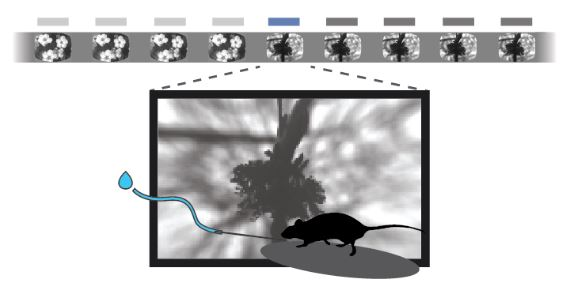
\includegraphics[width=133.56pt,height=76.26pt]{assets/mouse.JPG}};
%Straight Lines [id:da9493665930289801] 
\draw    (102.08,57.68) -- (102.08,66.08) ;

% Text Node
\draw (84.4,46) node [anchor=north west][inner sep=0.75pt]  [font=\footnotesize,color={rgb, 255:red, 74; green, 144; blue, 226 }  ,opacity=1 ] [align=left] {{\small Change}};
% Text Node
\draw (12.4,46.2) node [anchor=north west][inner sep=0.75pt]  [font=\footnotesize,color={rgb, 255:red, 74; green, 74; blue, 74 }  ,opacity=1 ] [align=left] {No change};


\end{tikzpicture}
        
        \caption*{ S$\Omega$I is used for  to estimate O-information for each $50 ms$ bin  of spikes recording intervals after the stimulus flash\cite{allen-inst}.}
    \end{figure}
\end{column}
\begin{column}{.5\textwidth}
\begin{figure}
\centering
    % \begin{subfigure}[]{0.4\textwidth}
    %     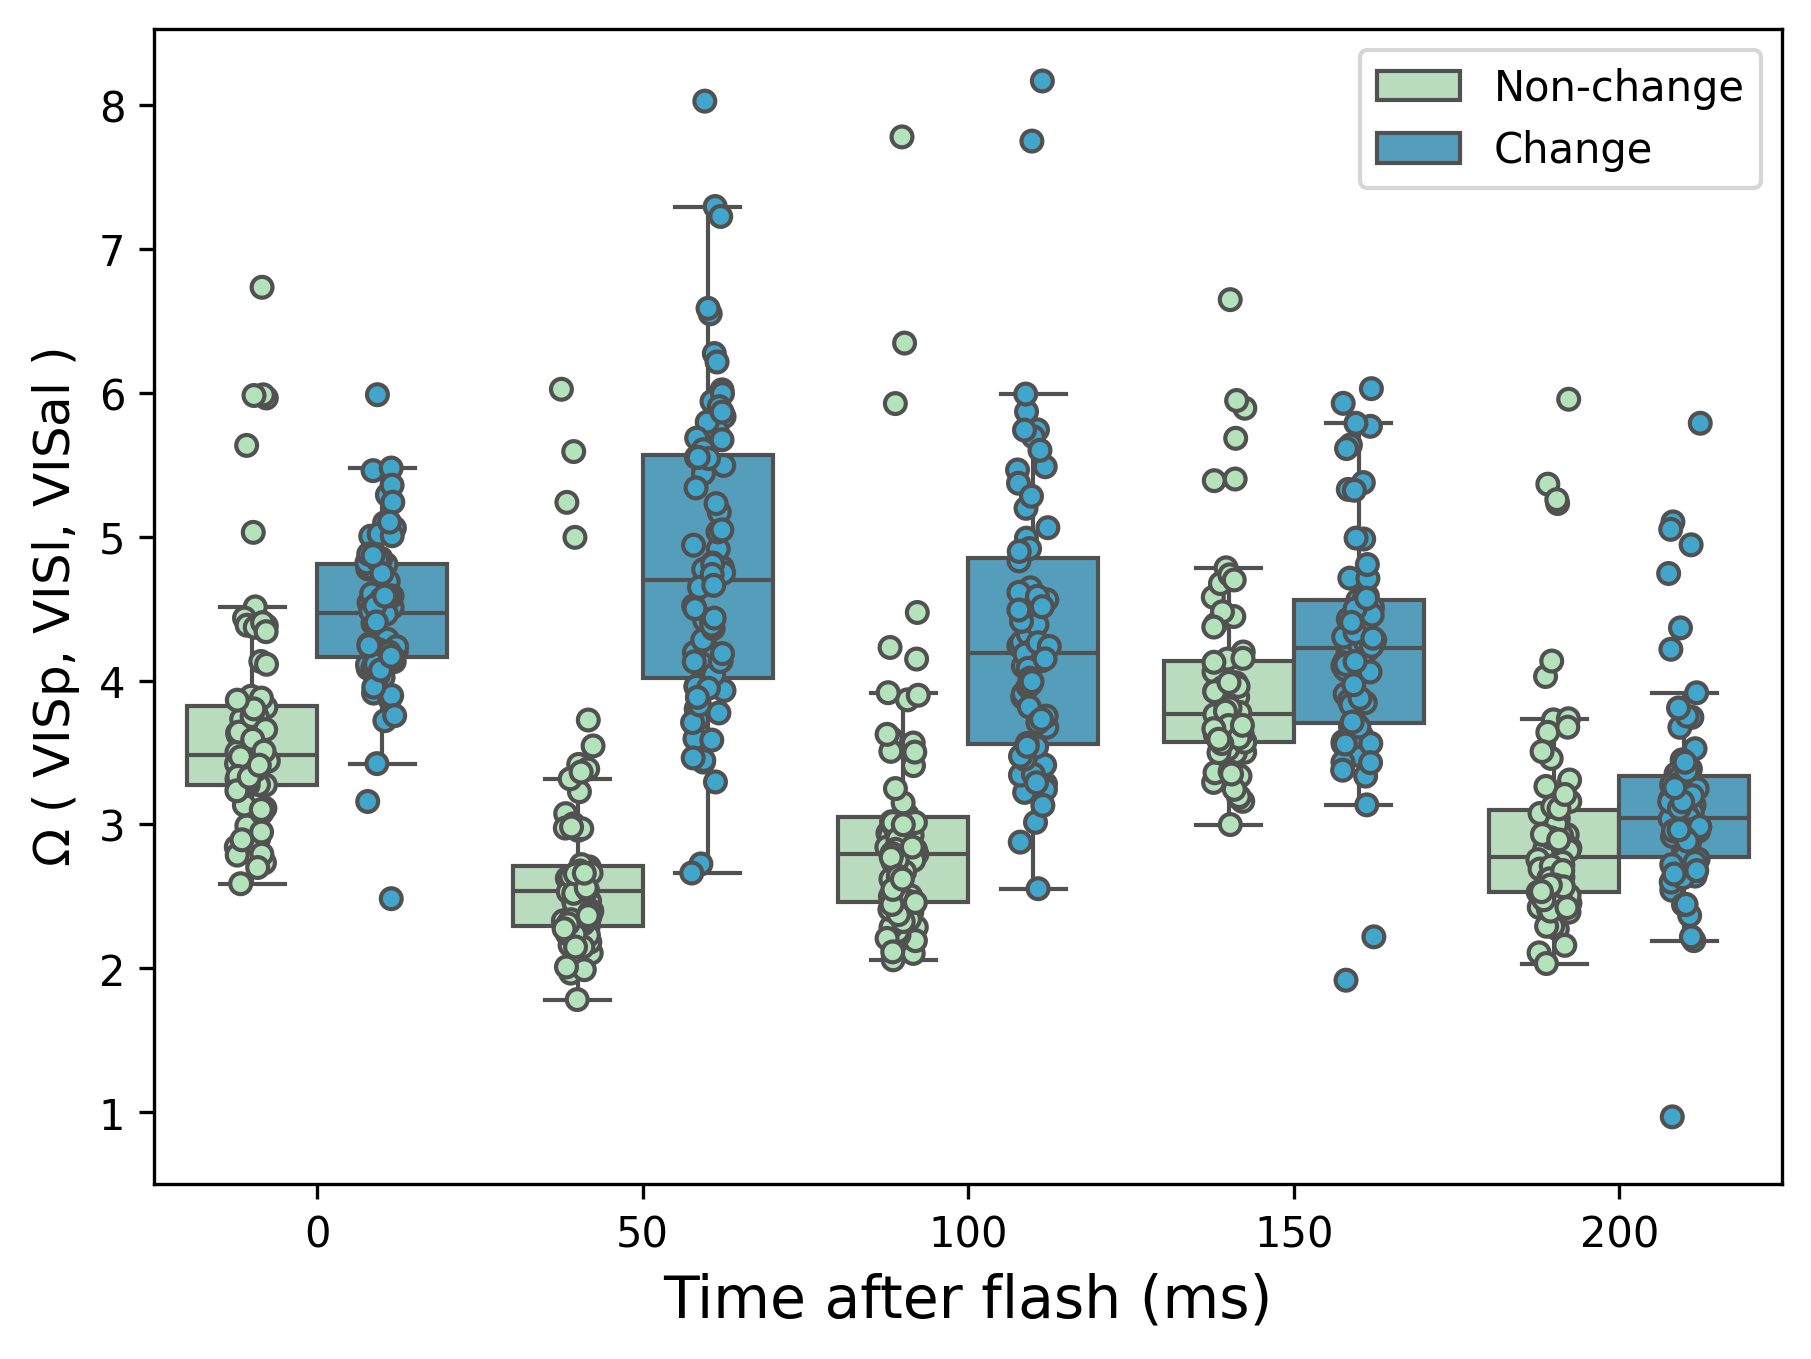
\includegraphics[width=\textwidth]{assets/figures/vbn/new_vbn_setting_3_dim_25.png}
    %     \caption*{3 brain regions}
    % \end{subfigure}
    \begin{subfigure}[]{0.8\textwidth}
        
\includegraphics[width=\textwidth]{assets/figures/vbn/new_vbn_setting_6_dim_25.png}
        \caption*{6 brain regions}
    \end{subfigure}
\caption*{ Higher \textbf{redundant} information in the visual cortex regions is transmitted in case of a flash with new scene.}

\end{figure}
\end{column}
\end{columns}
%% We applied our method to neural data from mice. The results showed higher redundancy in the visual cortex regions during specific stimuli, indicating the method's potential in neurobiological studies. This application demonstrates how SΩI can uncover intricate information dynamics in real biological systems.

\end{frame}

\begin{frame}{Conclusion}
\begin{itemize}
    \item S$\Omega$I captures high interaction information within multivariate information without restriction on the data distribution.
    \item S$\Omega$I opens the door for many scientific applications interested in analysing complex systems.
    \item Score based models for estimating information measures is a promising endeavour. 
\end{itemize}

\end{frame}


\begin{frame}{Thank you !}

 See you at the poster session number \textbf{..}.


\end{frame}



\end{document}
